\chapter{Technische Grundlagen}
\label{TechnischeGrundlagen}
\section{FlexSensor}
\label{tGl_FlexSensor}
\section{Balancing}
\label{tGl_Balancing}
\section{BLDC Motor}
\label{tGl_BLDC}

Für dieses Projekt wurde der Motor OX1 2-10 zur Verfügung gestellt. Dies ist ein dreiphasen Brushless DC-Motor ohne Hallsensoren. Die gegebenen technischen Daten sind in der Tabelle (Abbildung \ref{tabBLDCdaten}) ersichtlich. 
\todo{ref neben oben ... stehend u Referenz; in der nebenstehenden Tabelle} 
Des Weiteren ist am Motor ersichtlich, dass die Erregung aus 14 Permanentmagneten besteht und somit 7 Polpaare resultieren. Der Stator besteht aus 12 Spulen, somit ist jede Phase vier Mal gewickelt.
Der Aufbau entspricht einem Aussenläufermotor, ein BLDC-Motor verhält sich aus Regelungssicht wie eine permanenterregte Synchronmaschine. In der Abbildung \ref{figAufbauBLDC} ist das Feldverhalten dargestellt.\\

\begin{figure} [H]
%	\centering
	\subfigure[Prinzip Aufbau BLDC \cite{ElAntriebe_Babiel}]{
		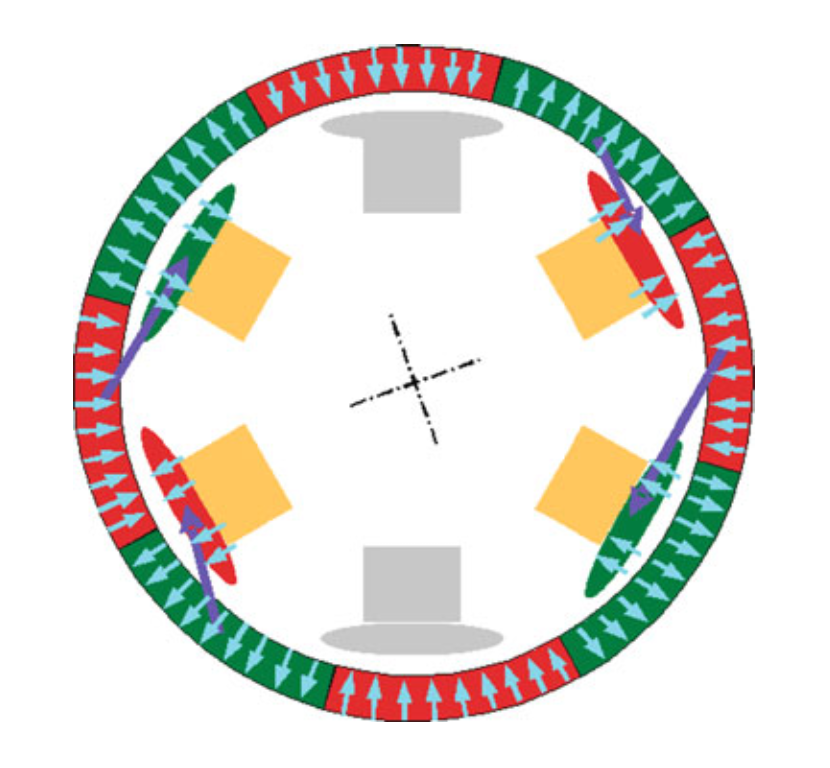
\includegraphics[width=0.45\linewidth]{images/AufbauBLDC} \label{figAufbauBLDC} 	}
	\subfigure[Sinstr][Sinusstrom mit PWM-Spannung \cite{InTech_PWM}]{ 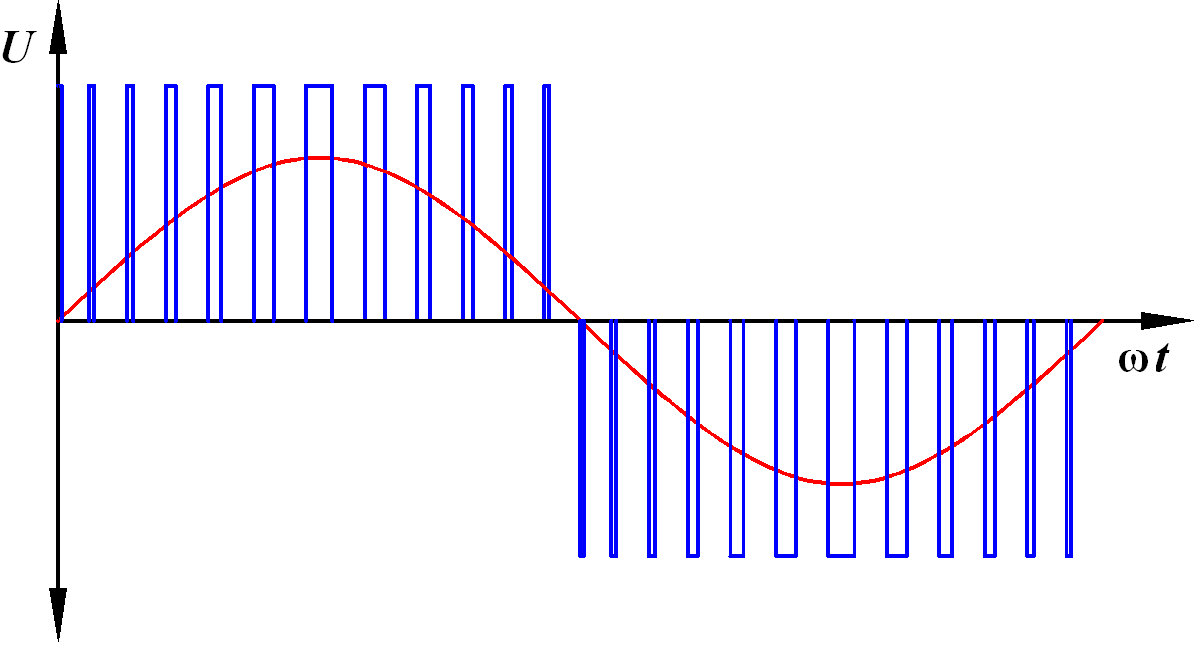
\includegraphics[width=0.5\linewidth]{images/StromBLDC} \label{figSinusstromPWM}}
	\caption[BLDC Motor]{Aufbau BLDC und PWM-Ansteuerung}
	\label{fig:BLDC}
\end{figure}

Angesteuert wird jede Phase über eine Halbbrücke. Die FOC-Regelungsweise (siehe Kapitel \ref{tGl_FOC}), setzt einen sinusförmigen Strom auf jeder Phase voraus, dies jeweils 120 Grad \todo{Grad-Zeichen einfügen %\textdegree \textcelcius ...} 
}Phasenverschoben. Realisiert wird dies mittels PWM-Ansteuerung der Halbbrücken. Da der Strom bei einer L-Last das Integral der Spannung ist, lässt sich ein quasi-sinusförmiger Strom generieren. Dargestellt ist dies in der Abbildung \ref{figSinusstromPWM}.

\begin{center}
	\begin{tabular}{|c|c|}
		\hline 
		\rule[-1ex]{0pt}{2.5ex}  BLDC Motor & Werte  \\ 
		\hline 
		\rule[-1ex]{0pt}{2.5ex} Idle Current & 1.2A \\ 
		\hline 
		\rule[-1ex]{0pt}{2.5ex} Max. Current & 50A \\ 
		\hline
		\rule[-1ex]{0pt}{2.5ex} Input Volt. & 2..10 x 3.6 Lipo (25.2V) \\ 
		\hline
		\rule[-1ex]{0pt}{2.5ex} Max. Output & 1815W \\ 
		\hline
		\rule[-1ex]{0pt}{2.5ex} Max. Pull & 6700g \\ 
		\hline
		\rule[-1ex]{0pt}{2.5ex} Rated Curren & 42.5A \\ 
		\hline
		\rule[-1ex]{0pt}{2.5ex} Motor Weight & 460g \\ 
		\hline
		\rule[-1ex]{0pt}{2.5ex} Shaft & 8mm \\ 
		\hline
		\rule[-1ex]{0pt}{2.5ex} Motor dimension & \O 50 x 65mm \\ 
		\hline
		\rule[-1ex]{0pt}{2.5ex} Internal Resistance & 0.0361$\Omega$ \\ 
		\hline	
	\end{tabular} 
	\captionof{figure}{BLDC Daten}
	\label{tabBLDCdaten}
\end{center}
\todo{e-Deutsch uebersetzung und Formatierung usw}
\todo{ev in Anhang??}

%\begin{figure} [H]
%	\centering
%	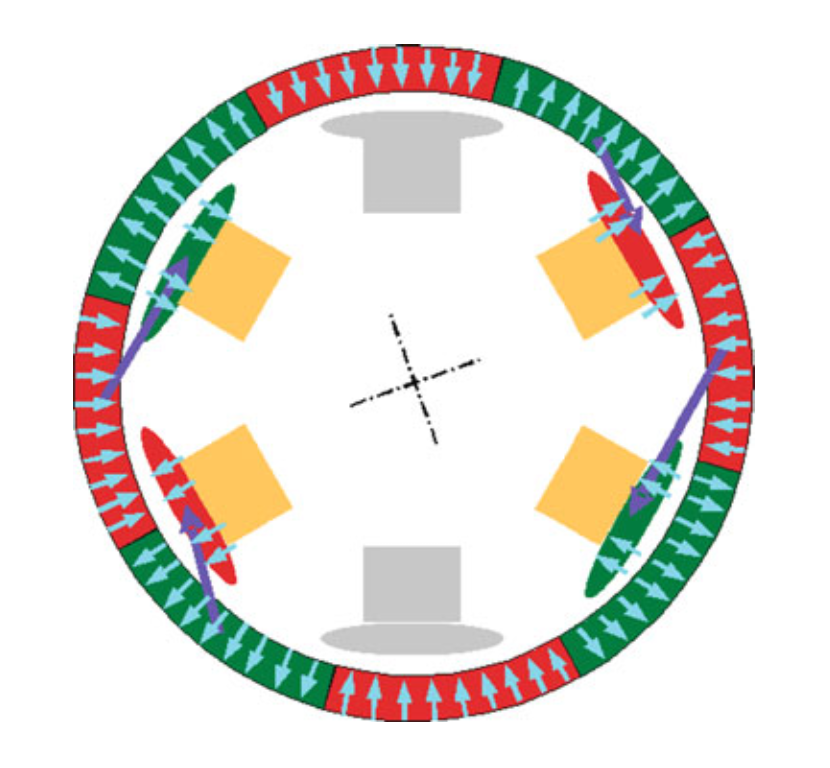
\includegraphics[width=0.4\linewidth]{images/AufbauBLDC}
%	\caption[Prinzip Aufbau]{Prinzip Aufbau}
%	\label{fig:aufbaubldc}
%\end{figure}

%\begin{figure} [H]
%	\centering
%	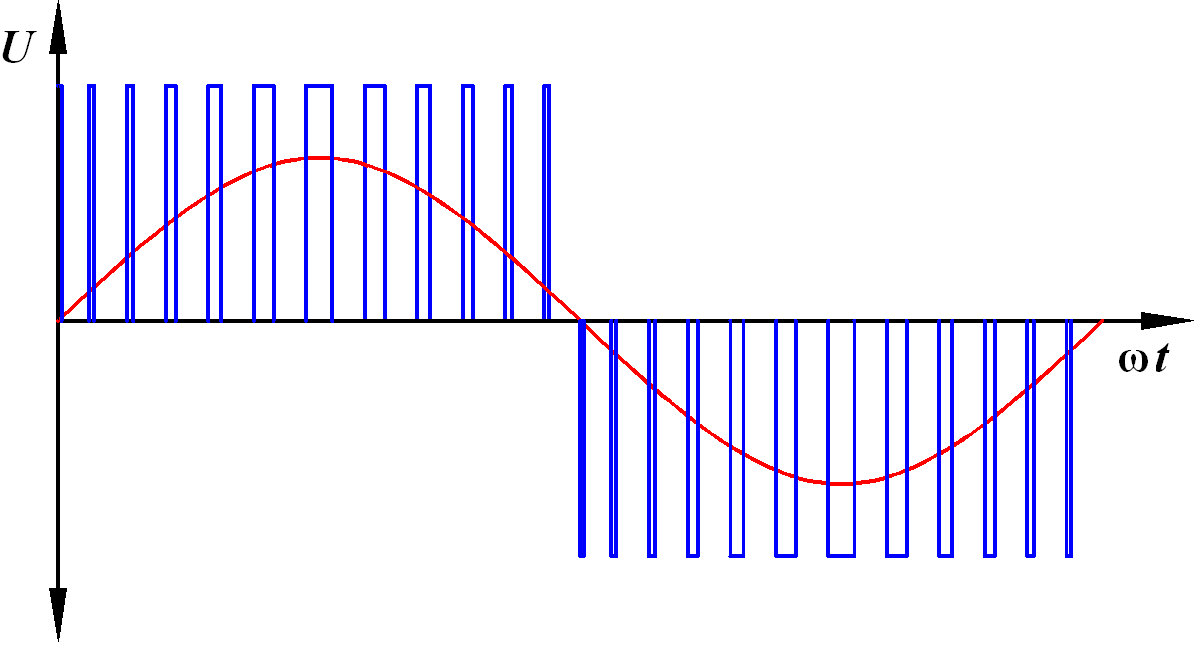
\includegraphics[width=0.5\linewidth]{images/StromBLDC}
%	\caption[Sinusstrom mit PWM Spannung]{Sinusstrom mit PWM Spannung}
%	\label{fig:strombldc}
%\end{figure}


\todo{\cite{ElAntriebe_Babiel} und korrekt zitieren...}


\section{FOC}
\label{tGl_FOC}
\section{FET, H-Brücke}
\label{tGl_HBrugg}
\section{Funkübertragung}
\label{tGl_RF}
